\begin{figure}
\begin{minipage}{0.65\linewidth}
    \centering
    \begin{tabular}{c}
        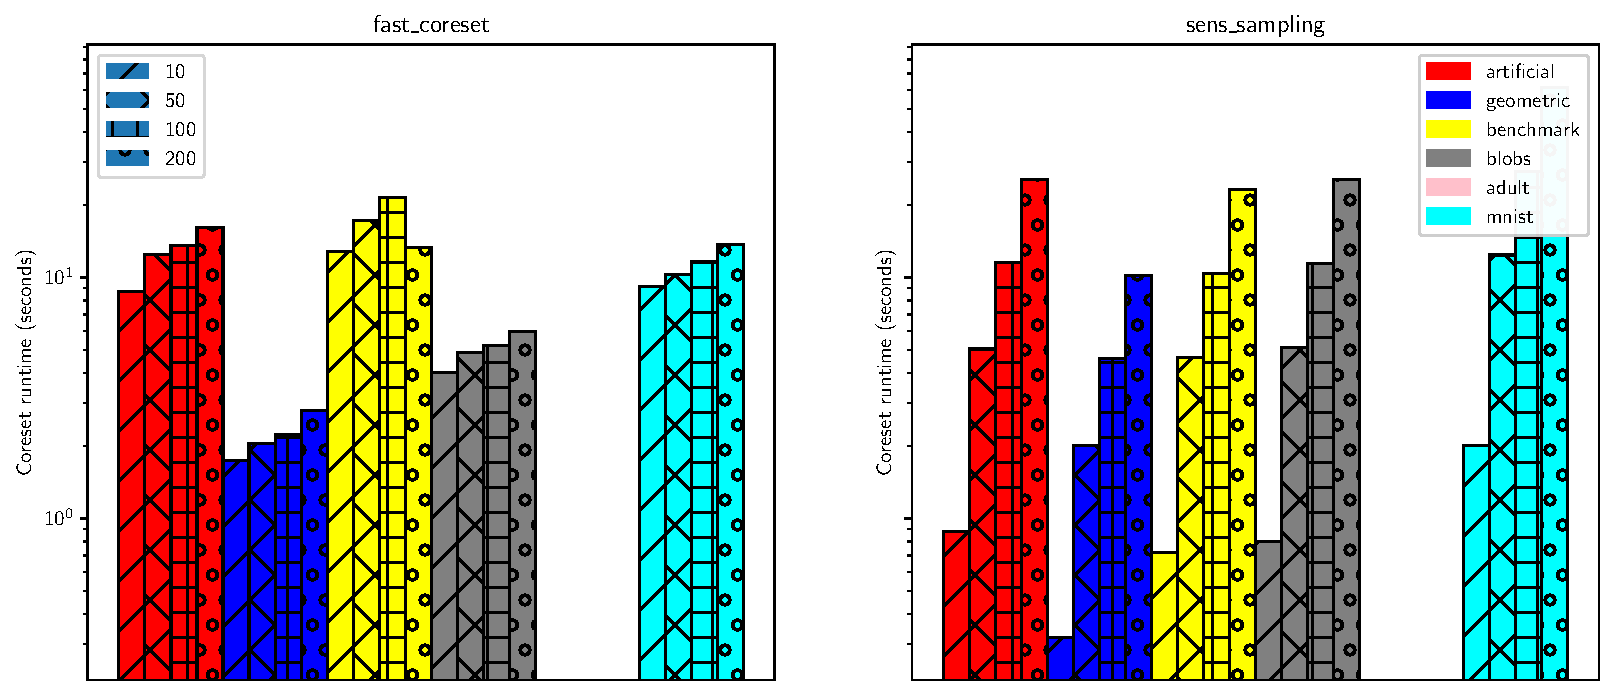
\includegraphics[width=.95\linewidth]{images/2/coreset_runtime-Effect_of_k_for_sens_sampling.pdf}
    \end{tabular}
    \caption{Mean runtime over five runs as we vary $k$ for sensitivity sampling and Fast-Coresets. Bars are $k=50, 100, 200, 400$; y-axis is log-scale.}
    \label{fig:coreset_size_on_sens_quality}
\end{minipage}
\hspace{0.35cm}
\begin{minipage}{0.27\linewidth}
    \centering
    \begin{tabular}{cc}
        Value of $r$ & Runtime \\
        \hline
        \vspace*{-0.2cm}\\
        20 & 13.5 $\pm$ 0.16 \\
        30 & 14.2 $\pm$ 0.33 \\
        40 & 15.5 $\pm$ 0.02 \\
        50 & 16.2 $\pm$ 0.16 \\
    \end{tabular}
    \captionof{table}{Mean runtime in seconds for \fkmeans as a function of $r \sim \log \Delta$, taken over five runs.}
    \label{tbl:logdelta}
\end{minipage}
\end{figure}
